\documentclass[tikz,border=4pt]{standalone}
% Paleta y fuentes compartidas por el libro y las figuras (única fuente de verdad).
\RequirePackage{xcolor}
\definecolor{oxido}{HTML}{B7410E}
\definecolor{cobre}{HTML}{D27D2D}
\definecolor{carbon}{HTML}{2B2B2B}
\definecolor{azul}{HTML}{1F5F8B}
\definecolor{arena}{HTML}{F4EDE4}

\usepackage{fontspec}
\setsansfont{FiraSans}[Extension=.otf,UprightFont=*-Regular,BoldFont=*-Bold,ItalicFont=*-Italic,BoldItalicFont=*-BoldItalic]
\setmonofont{FiraMono}[Extension=.otf,UprightFont=*-Regular,BoldFont=*-Medium]
\usetikzlibrary{positioning,arrows.meta,calc}
\begin{document}
\sffamily\small
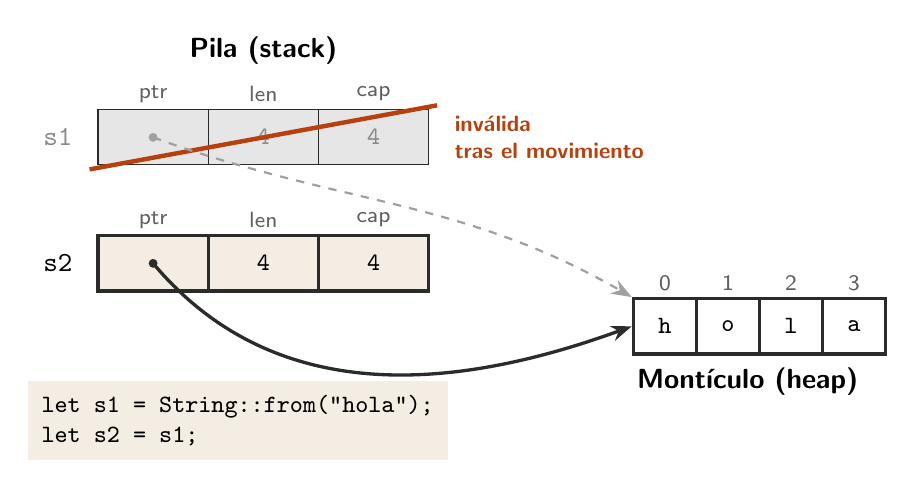
\begin{tikzpicture}[
  celda/.style={draw=carbon,minimum height=7mm,minimum width=14mm,font=\ttfamily\small},
  rotulo/.style={font=\sffamily\footnotesize\color{carbon!75}},
  >={Stealth[length=2.6mm]}]
  % Pila
  \node[font=\sffamily\bfseries] at (1.4,1.1) {Pila (\textit{stack})};
  \foreach \c/\v [count=\i from 0] in {ptr/{}, len/4, cap/4} {
    \node[celda,fill=carbon!12,text=carbon!55] (a\i) at (\i*1.4,0) {\v};
    \node[rotulo] at (\i*1.4,0.55) {\c};
    \node[celda,fill=arena,very thick] (b\i) at (\i*1.4,-1.6) {\v};
    \node[rotulo] at (\i*1.4,-1.05) {\c};
  }
  \node[anchor=east,font=\ttfamily\bfseries\color{carbon!55}] at (-0.9,0) {s1};
  \node[anchor=east,font=\ttfamily\bfseries] at (-0.9,-1.6) {s2};
  % s1 invalidada: tachado en diagonal + rótulo
  \draw[oxido,line width=1.6pt] ($(a0.south west)+(-0.1,-0.05)$) -- ($(a2.north east)+(0.1,0.05)$);
  \node[anchor=west,font=\sffamily\footnotesize\bfseries\color{oxido},align=left]
    at ($(a2.east)+(0.2,0)$) {inválida\\tras el movimiento};
  % Montículo
  \node[font=\sffamily\bfseries] at (7.55,-3.1) {Montículo (\textit{heap})};
  \foreach \l [count=\i from 0] in {h,o,l,a} {
    \node[celda,minimum width=8mm,fill=white,very thick] (h\i) at (6.5+\i*0.8,-2.4) {\l};
    \node[rotulo] at (6.5+\i*0.8,-1.85) {\i};
  }
  % Puntero válido de s2 (sólido) y antiguo de s1 (punteado)
  \fill[carbon] (b0.center) circle (1.6pt);
  \draw[->,very thick,carbon] (b0.center) to[out=-50,in=200] (h0.west);
  \fill[carbon!45] (a0.center) circle (1.6pt);
  \draw[->,thick,carbon!45,dashed] (a0.center) to[out=-20,in=150] (h0.north west);
  % Código
  \node[anchor=west,font=\ttfamily\small,align=left,fill=arena,inner sep=5pt]
    at (-1.6,-3.6) {let s1 = String::from("hola");\\let s2 = s1;};
\end{tikzpicture}
\end{document}
